\documentclass{wileySix}
\usepackage{w-bookps}

% \usepackage{mathptmx}

\usepackage{graphicx}
\usepackage{enumitem}

\setcounter{secnumdepth}{3}

\setcounter{tocdepth}{2}

\begin{document}

\booktitle{Sistem Operasi}
\subtitle{Semua Tentang Sistem Operasi}

\author{Rolly Maulana Awangga}

\halftitlepage
\titlepage



\offprintinfo{Sistem Operasi, pre-release}{Rolly Maulana Awangga}




\dedication{For my family}

\contentsinbrief %optional
\tableofcontents
\listoffigures %optional
\listoftables  %optional

%%%%%%%%%
%%Content 
%%%%%%%%%

\part[Pengenalan Sistem Operasi]
{Pengenalan\\ Sistem Operasi}

\chapter[Paging]
{Paging\\ Latex}

Kelompok : 4
Kelas : D4 TI 1A
Anggota : 
1. Damara Benedikta		1174012
2. Duvan Silalahi 		1174011
3. Ilham Habibi			1174028
4. Muhammad Fahmi		1174021
5. Oniwaldus Bere mali	1174005


\section { Sistem paging }
Sistem Paging Adalah sistem manajemen pada sistem operasi dalam mengatur program yang sedang berjalan. Program yang berjalan harus dimuat di memori utama. Kendala yang terjadi apabila suatu program lebih besar dibandingkan dengan memori utama yang tersedia.

Untuk mengatasi hal tersebut Sistem Paging mempunyai 2 solusi, yaitu:

\subsection {Konsep Overlay}
Dimana program yang dijalankan dipecah menjadi beberapa bagian yang dapat dimuat memori (overlay). Overlay yang belum diperlukan pada saat program berjalan (tidak sedang di eksekusi) disimpan di disk, dimana nantinya overlay tersebut akan dimuat ke memori begitu diperlukan dalam eksekusinya.

Konsep Memori Maya (virtual Memory)
Adalah kemampuan mengalamati ruang memori melebihi memori utama yang tersedia. Konsep ini pertama kali dikemukakan Fotheringham pada tahun 1961 untuk sistem komputer Atlas di Universitas Manchester, Inggris \ref{Gambar1}.

Gagasan Memori Maya adalah ukuran gabungan program, data dan stack melampaui jumlah memori fisik yang tersedia. Sistem operasi menyimpan bagian-bagian proses yang sedang digunakan di memori utama dan sisanya di disk. Begitu bagian di disk diperlukan maka bagian memori yang tidak diperlukan disingkirkan dan diganti bagian disk yang diperlukan.


	\begin{figure}[ht]
	\centerline{\includegraphics[width=1\textwidth]{figures/gambarpaging1.jpg}}
	\caption{Implementasi pemetaan memori system paging.}
	\label{Gambar1}
	\end{figure}

\section {Masalah Penggantian Halaman}

Berdasarkan pertimbangan tersebut, sebenarnya proses-proses yang memiliki 10 halaman hanya akan menggunakan setengah dari jumlah seluruh halaman yang dimilikinya. Kemudian demand paging akan menyimpan I/O yang dibutuhkan untuk mengisi 5 halaman yang belum pernah digunakan. Kita juga dapat meningkatkan derajat multiprogramming dengan menjalankan banyak proses sebanyak 2 kali.

\section {sistem paging }
pengertian sistem paging 
Sistem Paging Merupakan sistem yang memanajemen pada sistem operasi dalam mengelola program program yang sedang berjalan. Program program yang berjalan harus dimuat didalam memori utama. Batasan batasan yang terjadi saat program lebih besar dari memori utama yang telah tersedia. 
\cite{fomukong2003authorized}.

\subsection {pembagian solusi sistem paging }
a.Konsep Overlay
b.Konsep Memori Maya (virtual Memory)


\section {Masalah Penggantian Halaman }
 
Pada dasarnya, kesalahan halaman (page fault) sudah tidak lagi menjadi masalah yang terlalu  dianggap serius. Hal ini disebabkan karena masing-masing halaman pasti akan mengalami paling tidak satu kali kesalahan dalam pemberian halaman, yakni ketika halaman ini ditunjuk untuk pertama kalinya. Representasi seperti ini sebenarnya tidaklah terlalu akurat. 

a. Konsep Overlay
Dimana program yang dijalankan dipecah menjadi beberapa bagian yang dapat dimuat memori (overlay). Overlay yang belum diperlukan pada saat program berjalan (tidak sedang di eksekusi) disimpan di disk, dimana nantinya overlay tersebut akan dimuat ke memori begitu diperlukan dalam eksekusinya.

b. Konsep Memori Maya (virtual Memory)
Adalah kemampuan mengalamati ruang memori melebihi memori utama yang tersedia. Konsep ini pertama kali dikemukakan Fotheringham pada tahun 1961 untuk sistem komputer Atlas di Universitas Manchester, Inggris.

\section penggantian halaman
Pada dasarnya, kesalahan halaman tidak lagi menjadi masalah serius. Ini karena setiap halaman akan mengalami setidaknya satu kesalahan dalam pengiriman halaman, yaitu ketika halaman ini ditujukan untuk pertama kalinya. Representasi seperti ini sebenarnya tidak terlalu akurat. Berdasarkan pertimbangan ini, sebenarnya proses yang memiliki 10 halaman hanya akan menggunakan setengah dari jumlah total halaman yang dimilikinya. Kemudian permintaan paging akan menyimpan I / O yang diperlukan untuk mengisi 5 halaman yang belum pernah digunakan. Kami juga dapat meningkatkan tingkat multiprogramming dengan menjalankan beberapa proses 2 kali.

Lebih jauh lagi, kita harus mempertimbangkan bahwa sistem memori tidak hanya digunakan untuk menangani pengalamatan suatu program. Penyangga (buffer) untuk I/O juga menggunakan sejumlah memori. Penggunaan ini dapat meningkatkan pemakaian algoritma dalam penempatan di memori.

Beberapa sistem mengalokasikan secara pasti beberapa persen dari memori yang dimilikinya untuk penyangga I/O, dimana keduanya, baik proses

Lebih jauh lagi, kita harus mempertimbangkan bahwa sistem memori tidak hanya digunakan untuk menangani pengalamatan suatu program. Buffer untuk I / O juga menggunakan beberapa memori. Penggunaan ini dapat meningkatkan penggunaan algoritma dalam penempatan di memori.
Beberapa sistem mengalokasikan persis beberapa persen dari memori mereka untuk menyangga I / O, di mana keduanya,


Beberapa sistem mengalokasikan tepat beberapa persen dari memori mereka untuk buffer I / O, keduanya, baik proses pengguna dan subsistem I / O race untuk mengambil keuntungan dari seluruh sistem memori.

\section skema dasar pemindahan halaman 
Pemindahan halaman menggunakan pendekatan berikut. Jika tidak ada frame yang kosong, kami mencari frame yang tidak digunakan dan mengosongkannya. Kita dapat mengosongkan bingkai dengan menulis isinya ke dalam ruang swap, dan mengubah tabel halaman (serta tabel lainnya) untuk menunjukkan bahwa halaman tidak akan lama dalam memori.


\subsection cara memindahkan halaman

\begin{table}[H]
\begin{tabular}{|c|c|c|c|c|}
hline
No. & Nama & Jenis Kelamin & Pekerjaan & Alamat\\
\hline
1   & Cari lokasi dari halaman yang diinginkan pada disk
 & & &\\
2   & Cari frame kosong
 & & &\\
3   & Baca halaman yang diinginkan kedalam frame kosong yang baru & & &\\
4   & Ulang dari awal proses pengguna. & &\\
\hline
\end{tabular}
\end{table}

1. Cari lokasi dari halaman yang diinginkan pada disk

2. Cari frame kosong

a. Jika ada frame kosong, gunakan.
b. Jika tidak ada frame kosong, gunakan algoritma pemindahan halaman untuk menyeleksi frame yang akan digunakan.
c. Tulis halaman yang telah dipilih ke disk, ubah tabel halaman dan tabel frame.

3. Baca halaman yang diinginkan kedalam frame kosong yang baru, ubah tabel halaman dan tabel frame
 
4. Ulang dari awal proses pengguna.

Kita harus menyelesaikan 2 masalah utama untuk mengimplementasikan demand paging. Kita harus  mengembangkan algoritma pengalokasian rame dan algoritma pemindahan halaman. Jika kita memiliki banyak proses di memori, kita harus memutuskan berapa banyak frame yang akan dialokasikan ke masing-masing proses. Lebih jauh lagi, saat pemindahan halaman diinginkan, kita harus memilih frame yang akan dipindahkan. Membuat suatu algoritma yang tepat untuk menyelesaikan masalah ini adalah hal yang sangat penting.
ini adalah hal yang sangat penting.

Ada beberapa algoritma pemindahan halaman yang berbeda. Kemungkinan setiap Sistem Operasi memiliki skema pemindahan yang unik. Algoritma pemindahan yang baik adalah yang memiliki tingkat kesalahan halaman terendah. Kita mengevaluasi algoritma dengan menjalankanny dalam string khusus di memori acuan dan menghitung jumlah kesalahan halaman.  String dari memori acuan disebut string acuan (reference string). Sebagai contoh, jika kita memeriksa proses khusus, kita mungkin akan mencatat urutan alamat seperti dibawah ini:
0100, 0432, 0101, 0612, 0102, 0103, 0104, 0101, 0611, 0102, 0103, 0104, 0101, 0610, 0102, 0103,

0104, 0101, 0609, 0102, 0105, di mana pada 100 byte per halaman, diturunkan menjadi string referensi sebagai berikut:

1, 4, 1, 6, 1, 6, 1, 6, 1, 6, 1 

Perhatikan bahwa selama jumlah frame meningkat, jumlah kesalahan halaman menurun.

Penambahan memori fisik akan menambah jumlah frame.

\section Pemindahan Halaman Secara FIFO

Algoritma ini adalah algoritma paling sederhana dalam hal pemindahan halaman. Algoritma pemindahan


Pemindahan Halaman Secara FIFO

Algoritma ini adalah algoritma paling sederhana dalam hal pemindahan halaman. Algoritma pemindahan


Sebagai contoh:
Gambar 4-11. String Acuan. Sumber: . . .

7 0 1 2 0 3 0 4 2 3 0 3 2 1 2 0 1 7 0 1

7 7 7 2 2 2 4 4 4 0 0 0 7 7 7

0 0 0 3 3 3 2 2 2 1 1 1 0 0

1 1 1 0 0 0 3 3 3 2 2 2 1

Dari contoh contoh di atas, ada 15 halaman kesalahan. Algoritma FIFO mudah dimengerti dan diimplementasikan. Namun kinerjanya tidak selalu baik. Salah satu kelemahan dari algoritma FIFO adalah kemungkinan anomali Beladi, yang ada dalam beberapa kasus, tingkat kesalahan akan meningkat apabila jumlah frame yang dialokasikan juga meningkat.

\section pemindahan halaman secara optimal 
Salah satu konsekuensi mencegah anomali Beladi adalah algoritma pergerakan halaman yang optimal. Algoritma ini memiliki tingkat kesalahan halaman terendah dibandingkan dengan algoritma lainnya. Algoritma ini tidak akan mengalami anomali Belady. Konsep utama dari algoritma ini adalah mengganti halaman yang tidak akan digunakan untuk periode waktu terlama. Algoritma ini memastikan tingkat kesalahan serendah mungkin untuk sejumlah frame yang tetap.

\subsection Perlu disayangkan, algoritma optimal susah untuk diimplementasikan kedalam program, karena algoritma ini menuntut pengetahuan tentang string acuan yang akan muncul.

\section Pemindahan Halaman Secara LRU

Jika algoritma optimal sulit untuk dilakukan, mungkin kita dapat melakukan pendekatan terhadap algoritma tersebut. Jika kita menggunakan waktu yang baru berlalu sebagai pendekatan terhadap waktu yang akan datang, 

\subsection
(Least Recently Used) Rekan algoritma LRU dengan setiap halaman waktu dari halaman yang terakhir digunakan. Ketika halaman harus dipindahkan, LRU memilih halaman terpakai terpanjang di masa lalu. Berikut adalah algoritma LRU, lihat waktu lampau, bukan waktu yang akan datang.

Untuk mengimplementasikan algoritma LRU, ada 2 implementasi yang dapat digunakan, yaitu dengan counter dan stack. Selain algoritma optimal, algoritma LRU juga dapat menghindari anomali Beladi. Salah satu kelas algoritma halaman bergerak adalah algoritma tumpukan, yang juga tidak akan pernah mengalami anomali Beladi. Algoritma tumpukan ini menyimpan nomor halaman pada tumpukan. Kapan pun suatu halaman ditunjuk, halaman ini dikeluarkan dari tumpukan dan diletakkan di blok paling atas dari tumpukan. Dengan cara seperti ini, blok paling atas dari tumpukan selalu berisi halaman yang baru digunakan, sedangkan blok terbawah dari tumpukan selalu berisi halaman yang sudah lama tidak digunakan. Karena suatu halaman dalam tumpukan dapat dikeluarkan meski pun berada ditengah-tengah meski pun berada ditengah-tengah stack, maka implementasi terbaik untuk algoritma ini adalah dengan daftar mata rantai ganda ( doubly linked list), dengan kepala dan ekor sebagai penunjuk. Pendekatan ini sangat tepat untuk perangkat lunak atau implementasi kode mikro dari algoritma LRU.
 
\section Pemindahan Halaman Secara Perkiraan LRU

Awalnya, semua bit dikosongkan oleh sistem operasi. Selama proses pengguna, bit-bit yang terkait dengan setiap halaman referensi diatur ke 1 oleh perangkat keras. Setelah beberapa waktu, kami dapat menentukan halaman mana yang telah digunakan dan halaman mana yang belum digunakan dengan menguji bit referensi. Informasi ini memberikan informasi penting bagi banyak algoritma pemindahan halaman yang memperkirakan halaman mana yang tidak digunakan untuk waktu yang lama.
 
\section Algoritma Additional-Reference-Bit

Kita bisa mendapatkan informasi tambahan mengenai urutan dengan mencatat bit-bit acuan pada suatu interval yang tetap. Kita dapat menyimpan 8-bit byte untuk masing-masing halaman pada tabel di memori. Pada interval tertentu, pencatat waktu (timer) melakukan interupsi dengan mentransfer kontrol kepada sistem operasi. Sistem operasi mengubah bit acuan untuk masing-masing halaman kedalam bit high-order dari 8-bit byte ini dan membuang bit low-order. Register pengganti 8-bit ini berisi sejarah penggunaan halaman dalam periode 8 waktu terakhir.Sebagai contoh, seandainya register pengganti berisi 00000000, maka itu berarti halaman sudah tidak digunakan dalam periode 8 waktu terakhir, halaman yang digunakan paling tidak 1 kali akan memiliki nilai register penggati 11111111.

\section Algoritma second-chance
Algoritma second-chance didasarkan pada algoritma FIFO. Ketika sebuah halaman diarahkan, kita akan memeriksa bit referensi jika bit referensi adalah 0, kita memproses untuk menghapus halaman ini. Jika bit referensi adalah 1, kita memberikan kesempatan kedua. untuk halaman ini dan pilih halaman FIFO berikutnya.

Ketika halaman mendapat kesempatan kedua, bit referensi-nya akan dihapus dan waktu di-reset ke arus. Oleh karena itu, halaman yang mendapat kesempatan kedua tidak akan
dipindahkan sampai seluruh halaman dipindahkan. Selain itu, jika halaman yang digunakan cukup untuk menampung 1 set bit referensi, maka halaman ini tidak akan pernah dipindahkan.

\section Algoritme Second-Chance (Fixed)

Kita dapat memperbaiki kekurangan dari algoritma kesempatan kedua dengan mempertimbangkan 2 hal
sekaligus, bit referensi dan bit yang dimodifikasi. Dengan 2 bit ini, kita akan mendapatkan 4 kemungkinan
yang akan terjadi, yaitu:
• (0,0) tidak terpakai dan tidak dimodifikasi, sedikit terbaik untuk bergerak.

• (0,1) tidak digunakan tetapi dimodifikasi, tidak terlalu bagus untuk dipindahkan karena halaman ini perlu ditulis sebelum dipindahkan.

• (1.0) digunakan tetapi tidak dimodifikasi, mungkin halaman ini akan digunakan lagi segera.
 
• (1,1) digunakan dan dimodifikasi, halaman ini dapat segera digunakan lagi dan halaman ini harus ditulis ke disk sebelum dipindahkan. Algoritma ini digunakan dalam skema manajemen memori virtual Macintosh.


\chapter[Frekuensi Serial]
{frekuensiserial\\ Latex}
Kelompok : 4
Kelas : D4 TI 1A
Anggota : 
1. Damara Benedikta		1174012
2. Duvan Silalahi 		1174011
3. Ilham Habibi			1174028
4. Muhammad Fahmi		1174021
5. Oniwaldus Bere mali	1174005

\section {Frekuensi Serial}
Sebelum kita mengetahui apakah itu frekuensi serial, kita harus tau apakah defenisi dari frekuensi.
\subsection  {defenisi frekuensi}
Frekuensi adalah ukuran jumlah putaran ulang per peristiwa dalam satuan detik dengan satuan Hz.
Untuk menghitung frekuensi, seseorang menetapkan jarak waktu, menghitung jumlah kejadian peristiwa, dan membagi hitungan ini dengan panjang jarak waktu. Pada Sistem Satuan Internasional, hasil perhitungan ini dinyatakan dalam satuan hertz (Hz) yaitu nama pakar fisika Jerman Heinrich Rudolf Hertz yang menemukan fenomena ini pertama kali. Frekuensi sebesar 1 Hz menyatakan peristiwa yang terjadi satu kali per detik.
\section {Frekuensi Serial}
Pada frekuensi serial, setiap saat hanya dibutuhkan 1 bit data yang akan dikirim. Dengan kata lain, bit data akan dikirim satu per satu. frekuensi ini memiliki keuntungan yang hanya membutuhkan satu jalur dan beberapa kabel dibandingkan dengan komunikasi paralel. Pada prinsipnya frekuensi serial adalah frekuensi di mana transmisi data dilakukan per bit sehingga lebih lambat daripada frekuensi paralel, atau dengan kata lain frekuensi serial adalah salah satu metode komunikasi data dimana hanya satu bit data yang dikirimkan melalui seutas kabel pada waktu tertentu.
<<<<<<< HEAD
\section {Frekuensi serial adalah frekuensi yang pengiriman datanya per-bit secara berurutan dan bergantian. Frekuensi ini mempunyai suatu kelebihan yaitu hanya membutuhkan satu jalur dan kabel yang sedikit dibandingkan dengan komunikasi paralel. Pada prinsipnya komunikasi serial merupakanfrekuensi dimana pengiriman data dilakukan per bit sehingga lebih lambat dibandingkan frekuensi parallel, atau dengan kata lain komunikasi serial merupakan salah satu metode komunikasi data di mana hanya satu bit data yang dikirimkan melalui seuntai kabel pada suatu waktu tertentu. Pada dasarnya komunikasi serial adalah kasus khusus komunikasi paralel dengan nilai n = 1, atau dengan kata lain adalah suatu bentuk komunikasi paralel dengan jumlah kabel hanya satu dan hanya mengirimkan satu bit data secara simultan.
\subsection {Hal ini dapat disandingkan dengan komunikasi paralel yang sesungguhnya di mana n-bit data dikirimkan bersamaan, dengan nilai umumnya 8 ≤ n ≤ 128.
=======
<<<<<<< HEAD

\section {ada 2 jenis}
Komunikasi serial terdiri dari dua jenis, serial serial dan sinkron asynchronous. Serial sinkron adalah komunikasi di mana hanya ada satu pihak (pengirim atau penerima) yang menghasilkan jam dan mengirim jam bersama dengan data. Contoh penggunaan serial sinkron ada pada transmisi data keyboard. Asynchronous serial adalah komunikasi di mana kedua pihak (pengirim dan penerima) masing-masing menghasilkan clock tetapi hanya data yang ditransmisikan, tanpa jam. Agar data yang akan ditransmisikan menjadi sama dengan data yang diterima, kedua frekuensi clock harus sama dan harus disinkronkan. Setelah sinkronisasi, pengirim akan mengirim data sesuai dengan frekuensi jam pengirim dan penerima akan membaca data sesuai dengan frekuensi jam penerima. Contoh penggunaan serial asynchronous adalah pada Universal Asynchronous Receiver Transmitter (UART) yang digunakan pada komputer port serial (COM)

=======
\section {serial mode}
Mode serial memerlukan sinkronisasi atau penyesuaian yang berfungsi untuk:
\subsection {fungsi sinkronisasi}
Mengetahui kapan sinyal yang diterimanya adalah sedikit data (bit sinkronisasi)
Mengetahui kapan sinyal yang diterimanya membentuk karakter (sinkronisasi karakter)
Mengetahui kapan sinyal yang diterimanya membentuk blok data (memblokir sinkronisasi)
Selanjutnya, transmisi serial dapat mengambil bentuk dua jenis, yaitu transmisi serial sinkron (sinkron) dan transmisi serial asynchronous (asynchronous). Berikut ini adalah penjelasan dari masing-masing jenis transmisi serial. 
\section Transmisi Serial Sinkron, pengirim akan mengirimkan datanya sesuai dengan frekuensi clock pengirim dan penerima akan membaca data sesuai dengan frekuensi clock penerima. Contoh penggunaan asynchronous serial adalah pada Universal Asynchronous Receiver Transmitter (UART) yang digunakan pada serial port (COM) komputer.
\subsection Antarmuka Kanal serial lebih kompleks/sulit dibandingkan dengan antarmuka melalui
kanal paralel, hal ini disebabkan karena:
\section 1. Dari Segi perangkat keras: adanya proses konversi data pararel menjadi serial atau sebaliknya menggunakan piranti tambahan yang disebut UART (Universal Asynchronous Receiver/Transmitte) dan
2. Dari Segi perangkat lunak: lebih banyak register yang digunakan atau terlibat
\subsection Namun di sisi lain antarmuka kanal serial menawarkan berapa kelebihan dibandingkan secara paralel, antara lain:

>>>>>>> da5ec7e8faaa61dff7bd70ec0b7ddb225ceb48f7
>>>>>>> 546699ff1b4072148b1d901996329551145c5c85

1. Dari Segi perangkat keras: adanya proses konversi data pararel menjadi serial atau sebaliknya menggunakan piranti tambahan yang disebut UART (Universal Asynchronous Receiver/Transmitte) dan
2. Dari Segi perangkat lunak: lebih banyak register yang digunakan atau terlibat
Namun di sisi lain antarmuka kanal serial menawarkan berapa kelebihan dibandingkan secara paralel, antara lain:


1. Kabel untuk komunikasi serial bisa lebih panjang dibandingkan dengan paralel; data-data dalam komunikasi serial dikirim-kan untuk logika ‘1’ sebagai tegangan -3 s/d -25 volt dan untuk logika ‘0’ sebagai tegangan +3 s/d +25 volt, dengan demikian tegangan dalam komunikasi serial memiliki ayunan tegangan maksimum 50 volt, sedangkan pada komunikasi paralel hanya 5 volt. Hal ini menyebabkan gangguan pada kabel-kabel panjang lebih mudah diatasi dibandingkan pada parallel.
15:35 ONI Banyak mikrokontroler yang Namun pada masing-masing komputer dengan komunikasi serial harus dibayar “biaya” antarmuka serial yang agak lebih mahal.
2. Jumlah kabel serial lebih sedikit; Anda bisa menghubungkan dua perangkat komputer yang berjauhan dengan hanya 3 kabel untuk konfigurasi null modem, yaitu TXD (saluran kirim), RXD(saluran terima) dan Ground, bayangkan jika digunakan teknik paralel akan terdapat 20 – 25 kabel. Namun pada masing-masing komputer dengan komunikasi serial harus dibayar “biaya” antarmuka serial yang agak lebih mahal.

3. Banyaknya piranti saat ini (palmtop, organizer, hand-phone dan lainlain) menggunakan teknologi infra merah untuk komunikasi data, dalam hal ini pengiriman datanya dilakukan secara serial. IrDA-1 (spesifikasi infra merah pertama) mampu mengirimkan data dengan laju 115,2 kbps
15:35 ONI dan Konsep Komunikasi Serial 2 dibantu dengan piranti UART, hanya panjang pulsa berkurang menjadi 3/16 dari standar RS-232 untuk menghemat daya.









\section {Pengertian Port}
PENGERTIAN  PORT
Port merupakan satu set perintah yang digunakan oleh komputer untuk memindahkan data dari atau ke perangkat lain, misalnya untuk berhubungan dengan keyboard, mouse, printer, modem, monitor dan sebagainya. Ada berbagai macam port, yaitu :
·         Serial Port
·         Pararel Port
·         IDE
·         SATA
·         USB
·         Ethernet
·         Audio Codec
·         PCI

\section {SERIAL PORT }

	\begin{figure}[ht]
	\centerline{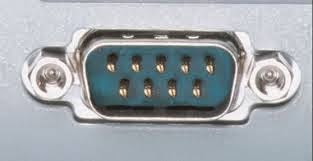
\includegraphics[width=1\textwidth]{figures/port1.jpg}}
	\caption{Implementasi pemetaan memori system paging.}
	\label{Gambar1}
	\end{figure}

	\begin{figure}[ht]
	\centerline{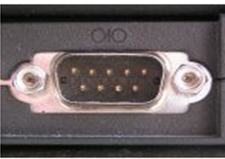
\includegraphics[width=1\textwidth]{figures/port2.jpg}}
	\caption{Implementasi pemetaan memori system paging.}
	\label{Gambar2}
	\end{figure}

\subsection{Pengertian dan Fungsi Serial Port}\ref{Gambar1}
Serial Port atau biasa disebut dalam bahasa Indonesia adalah port seri merupakan sebuah port pada personal computer yang berfungsi untuk mentransmisikan satu bit informasi pada satu satuan waktu. Dalam serial port, pengiriman informasi tidak memungkinkan untuk melakukan secara banyak sekalius. Hal ini disebabkan karena dalam melakukan pemindahan data, biasanya serial port bekerja seri, misalnya COM 1 dan COM 2. Untuk penggunaan port serial sekarang ini sudah berkurang. Penggunaan port serial telah tergantikan dengan port USB dan Firewire. Sedangkan untuk jaringan (networking) fungsinya sudah tergantikan dengan port Ethernet. Berikut beberapa fungsi serial port yaitu menghubungkan antara peripheral (alat) computer lain dengan motherboard, penghubung antara mouse dengan motherboard, penghubung antara modem dengan motherboard, dan mentransmisikan informasi-informasi berupa bit-bit dari mainboard ke perangkat lainnya. Konektor yang digunakan adalah RS-232C dengan 9 pin atau 25 pin. \ref{Gambar2}.

\section {dasar-dasar komunikasi serial}
Saat di mana komputer berkomunikasi dengan dunia luar, semua dilakukan dengan data berukuran byte. Dan hal yang sama, seperti printer, informasi data langsung dilakukan melalui data BUS 8-bit ke 8-bit BUS dari data printer. Ini dapat bekerja selama jaraknya tidak terlalu jauh, mengingat jarak kabel yang panjang akan mengurangi (mengganggu) kualitas sinyal. Kabel yang buruk dan sangat panjang akan membuat logika palsu, dan data menjadi tidak perlu diubah.
<<<<<<< HEAD

\section 
Selain itu, hubungan data 8-bit menjadi sangat mahal, karena dibutuhkan kualitas kabel yang sangat baik dan jumlah yang lebih banyak. Untuk alasan ini, komunikasi serial digunakan untuk mentransfer data antara dua sistem dengan jarak yang sangat jauh mulai dari beberapa puluh meter hingga ribuan kilometer. Gambar 10-1 menunjukkan grafik transfer data serial dan paralel.

\subsection { dasar komunikasi serial }
a. Komunikasi Half- dan Full-Duplex
b. Komunikasi serial Asynchronous dan Data Framing

=======
\subsection {framing data}
Framing data adalah bagaimana suatu rangkaian bit disusun untuk dikirim melalui suatu sistem komunikasi serial.Data yang dikirim melalui komunikasi serial biasanya adalah 5 sampai 9-bit. Pada Arduino, data berukuran sebesar 8-bit (1-byte).
Start dan Stop bit dikenal sebagai synchronization bit. Start dan Stop bit bisa berukuran 2 atau 3-bit. Sesuai dengan namanya, bit-bit ini akan mengawali dan mengakhiri paket data. Start bit selalu berukuran 1-bit, sedangkan Stop bit bisa 1 atau 2-bit. Jika tidak diperlukan untuk dikonfigurasi, biarkan saja nilai Stop bit sebesar 1-bit.

\section {Generasi Serial Port}
PS/2. PS2 merupakan perkembangan dari port serial. Bentuknya berupa bulatan dengan desain sedemikian rupa sehingga tidak mungkin terbalik atau salah. Komputer dengan processor pentium MMX ke atas biasanya terdapat 2 port PS2, yaitu untuk mouse dan keyboard.
Namun saat ini penggunaan port serial sebagain besar sudah digantikan oleh jenis port baru yang bernama USB. Saat ini USB sudah benar-benar diterima pasar dan menggantikan kepopuleran port serial dan port parallel. Saat ini jika kita butuh serial port jenis RS232 atau paralel port(printer port) di sebuah komputer, maka pada saat membeli komputer kita harus memeriksa terlebih dahulu apakah motherboardnya menyediakan serial port dan paralel port. Sedangkan untuk mencari motherboard dengan USB board bukanlah hal yang sulit, umumnya setiap motherboard saat ini telah dilengkapi dengan 2 hingga 4 buah slot port USB dan dua lagi tambahan port USB di bagian depan casing CPU.
<<<<<<< HEAD
>>>>>>> 1cfae4b86747c1021e2d43703f1c095f5aaaaa60
=======
>>>>>>> 3fc5fab8ee52b853c5c2af711c1a02eb8ae20252

\section{Karakteristik Sinyal Serial Port}
Standar sinyal komunikasi serial yang paling umum digunakan adalah standar RS232. Standar ini hanya melibatkan komunikasi data antara komputer (Data Terminal Equipment - DTE) dengan komputer - peralatan bantu (Data Circuit - Terminating Equipment - DCE). Standarad RS232 umumnya digunakan pada port serial IBM PC Compatible.
\subsection{level standart sinyal }
a. Logika '1' disebut 'mark' yang terletak antara -3 volt hingga -25 volt.
b. Logika '0' disebut 'ruang' yang terletak di antara +3 volt hingga +25 volt.
Area tegangan antara -3 volt hingga +3 volt adalah level yang tidak valid, yaitu area voltase yang tidak memiliki level logika harus dihindari. Demikian pula tingkat tegangan negatif -25 volt atau lebih positif dari +25 volt juga harus dihindari karena dapat merusak driver garis pada jalur RS232.

\section{Konfigurasi serial port}
Untuk dapat menggunakan port serial
itu. Biasanya tersedia dua port serial pada CPU, yaitu COM1 dan COM2. Mendasarkan
Alamat COM1 biasanya 1016 (3F8h) dan COM2 biasanya 760 (2F8h). Alamat
adalah alamat biasa, tergantung pada komputer yang tepat milik kita
dapat melihat di peta memori, yaitu memori
0000.0400h untuk COM1 dan 0000.0402h untuk COM2.
\section {Alasan Penggunaan Port Serial}
Dibandingkan dengan menggunakan port parallel penggunaan port serial terkesan lebih rumit. Berikut adalah keuntungan penggunaan port serial dibandingkan penggunaan port parallel.
\subsection 1.Pada komunikasi dengan kabel yang panjang, masalah cable loss tidak akan menjadi masalah besar daripada menggunakan kabel parallel. Port serial mentransmisikan “1” pada level tegangan -3 Volt sampai -25 Volt dan “0” pada level tegangan +3 Volt sampai +25 Volt, sedangkan port parallel mentransmisikan “0” pada level tegangan 0 Volt dan “1” pada level tegangan 5 Volt. 
\section 2. Dubutuhkan jumlah kabel yang sedikit, bisa hanya menggunakan 3 kabel yaitu saluran Transmit Data, saluran Receive Data, dan saluran Ground (Konfigurasi Null Modem 
  \subsection 3. Saat ini penggunaan mikrokontroller semakin populer. Kebanyakan mikrokontroller sudah dilengkapi dengan SCI (Serial Communication Interface) yang dapat digunakan untuk komunikasi dengan port serial komputer

<<<<<<< HEAD
 
=======
 \section UART(Universal Asincrhounus Recivier transmiter)
UART atau Universal Asynchronous Receiver-Transmitter adalah bagian perangkat keras komputer yang menerjemahkan antara bit-bit paralel data dan bit-bit serial. UART biasanya berupa sirkuit terintegrasi yang digunakan untuk komunikasi serial pada komputer atau port serial perangkat periperal. UART sekarang ini termasuk di dalam beberapa mikrokontroler (contohnya, PIC16F628).
Komponen keping UART tipikal
Keping UART biasanya terdiri dari:
·         Penyangga (buffer) Transmit/Receive 
·         Pengendali (control) Transmit/Receive 
·         Penyangga Bus Data 
·         Logika Kendali Read/Write 
·         Kendali Modem 
>>>>>>> 253ba8571fcc632a051bb2db2e5a2f851f3018e8
\section {Penjelasan UART}
UART atau Universal Asynchronous Receiver Transmitter adalah protokol komunikasi yang umum digunakan untuk mentransmisikan data serial antar perangkat satu dengan lainnya. Misalnya komunikasi antar sesama mikrokontroler atau mikrokontroler ke PC. Dalam transmisi data, jam antara pengirim dan penerima harus sama karena paket data dikirim setiap bit bergantung pada jam. Ini adalah salah satu keuntungan dari model asynchronous dalam transmisi data karena hanya dengan satu kabel transmisi data dapat ditransmisikan. Berbeda dengan model sinkron yang terdapat dalam protokol SPI (Serial Peripheral Interface) dan I2C (Inter-Integrated Circuit) karena protokolnya membutuhkan setidaknya dua kabel dalam transmisi data, yaitu clock dan transmisi data. Namun kelemahan model asynchronous adalah dalam hal kecepatan dan jarak transmisi. Karena transmisi jarak yang lebih cepat dan jauh membuat paket data bit menjadi terdistorsi sehingga data yang dikirim atau diterima dapat memiliki kesalahan.


%\chapter[Internet]
%{Definisi\\ Internet}
%\input{section/1internet.tex}

%\chapter[Web]
%{Definisi\\ Web}
%\input{section/1web.tex}

%\chapter[Backend]
%{Definisi\\ Backend}
%\input{section/1Backend.tex}

%\chapter[Frontend]
%{Definisi\\ Frontend}
%\input{section/1Frontend.tex}

% contoh aplikasi web service
% web service
% protokol
% port

% HTTP
% URL
% POST
% GET


\bibliographystyle{IEEEtran}
\bibliography{references}

\printindex

\end{document}
